\documentclass[10pt,a4paper]{article}
\usepackage{amsmath,amssymb,amsthm,graphicx}
\usepackage{graphicx}
\providecommand{\ket}[1]{\lvert#1\rangle}
\providecommand{\bra}[1]{\langle#1\rvert}
\providecommand{\proj}[1]{\ket{#1}\bra{#1}}
\providecommand{\Id}[1]{\mathbf1_{#1}}
\providecommand{\QAliceRest}{X_{\overline C}\widetilde X_{\overline C}A}
\providecommand{\QBobRest}{Y_{\overline C}\widetilde Y_{\overline C}BZ_{\overline C}}
\providecommand{\QAllRest}{X_{\overline C}\widetilde X_{\overline C}Y_{\overline C}\widetilde Y_{\overline C}ABZ_{\overline C}}
\title{Strong direct product for entanglement-assisted one-way quantum communication}
\author{Rahul Jain, Srijita Kundu}
\date{doi:10.4230/LIPIcs.CCC.2021.27; CC BY4.0}
\begin{document}
\maketitle
\noindent\textit{Editorial note.} Original authors: Rahul Jain and Srijita Kundu. Official CCC2021 article27 (2021-07-08), DOI10.4230/LIPIcs.CCC.2021.27.\par\medskip
\noindent\textit{Editorial note.} License: https://creativecommons.org/licenses/by/4.0/\par\medskip
\noindent\textit{Editorial note.} Faithful editable TeX collection of formal author Theorem1, complete Section3 anchoring/distribution/protocol construction and Lemma30/31/32 proofs including all information, projector, unitary, channel and final coordinate-selection continuation. Required exact probability/CQ-state facts, local conditioning and substate proof, communication model and prior compression/embedding facts are retained with their original conditions. Original Figure1 is cropped from the official PDF as a diagram asset, not a source-page substitute. Full published bibliography retained. Typographic macros expand to the original register bundles. Author mathematical expressions and conditions are uncorrected; no new proof or assumptions. Only official CC BY4.0 content used; arxiv2008.08963/ECCC are identity aliases, and related arxiv2106.04299 is not an alias.\par\medskip
\noindent\textit{Allowed standard prerequisites (editorial).}\begin{itemize}
\item Quantum substate, Uhlmann and Quantum Raz lemmas. Exact author Facts13--24 and stated hypotheses retained.
\item Measurement-based message compression. Exact Fact25[29] with full author explanation of the adapted register/entropy formulation retained.
\item Classical embedding and minimax. Exact Facts10/12[19,25], Fact28[45] and local conditioning proofs retained.
\end{itemize}\medskip
\section*{Author Section 2.1: probability theory}
The probability distribution of $X$ is $P_X$, and conditioned on an event $E$ it is $P_{X|E}$. $P_{X|Y=y}$ may be abbreviated $P_{X|y}$. The product notation $P_{XY}P_{Z|X}$ means $(P_{XY}P_{Z|X})(x,y,z)=P_{XY}(x,y)P_{Z|X=x}(z)$. The $\ell_1$ distance is $\|P_X-P_{X'}\|_1=\sum_x|P_X(x)-P_{X'}(x)|$.
\paragraph{Fact 4.} For joint distributions on the same sets, $\|P_X-P_{X'}\|_1\le\|P_{XY}-P_{X'Y'}\|_1$.
\paragraph{Fact 5.} For an event $E$, $|P_X(E)-P_{X'}(E)|\le\frac12\|P_X-P_{X'}\|_1$.
\paragraph{Fact 6.} For a coupling $P_{XX'}$ with marginals $P_X,P_{X'}$, $\|P_X-P_{X'}\|_1\le2P_{XX'}(X\ne X')$.
\paragraph{Fact 7.} If $\|P_X-P_{X'}\|_1\le\epsilon$ and $P_X(E)\ge\alpha>\epsilon$, then $\|P_{X|E}-P_{X'|E}\|_1\le2\epsilon/\alpha$.
\begin{proof}Fact5 gives $\alpha-\epsilon/2\le P_{X'}(E)\le\alpha+\epsilon/2$. There is $E'$ with $2(P_{X|E}(E')-P_{X'|E}(E'))=\|P_{X|E}-P_{X'|E}\|_1$. Also $P_X(E\wedge E')=P_X(E)P_{X|E}(E')\ge\alpha P_{X|E}(E')$, and $P_{X'}(E\wedge E')\le(\alpha+\epsilon/2)P_{X'|E}(E')\le\alpha P_{X'|E}(E')+\frac12\|P_X-P_{X'}\|_1$. Thus
\begin{align*}\|P_X-P_{X'}\|_1&\ge2(P_X(E\wedge E')-P_{X'}(E\wedge E'))\\&\ge2\alpha(P_{X|E}(E')-P_{X'|E}(E'))-\|P_X-P_{X'}\|_1\\&\ge\alpha\|P_{X|E}-P_{X'|E}\|_1-\|P_X-P_{X'}\|_1,\end{align*}
giving the result.\end{proof}
\paragraph{Fact 8 ([3],Lemma16).} If $P_{XY}(x,y^*)=\alpha P_X(x)$ for every $x$, then
\[\|P_{XYZ}-P_{XY}P_{Z|X,y^*}\|_1\le\frac2\alpha\|P_{XYZ}-P_{XY}P_{Z|X}\|_1.\]
\paragraph{Corollary 9.} Suppose $P_{XY}$ and $P_{X'Y'Z'}$ satisfy $P_X(x,y^*)=\alpha P_X(x)$ for all $x$. Then
\[\|P_{X'Z'|y^*}-P_{X'Z'}\|_1\le\frac{11}\alpha\|P_{X'Y'Z'}-P_{XY}P_{Z'|X'}\|_1.\]
\begin{proof}Let the norm on the RHS be $\epsilon$. Fact7 gives $\|P_{X|y^*}-P_{X'|y^*}\|_1\le2\epsilon/\alpha$. Let $P_{XYZ''}=P_{XY}P_{Z'|X'Y'}$. Then
\begin{align*}\|P_{X'Z'}-P_{XZ''}\|_1&=\sum_{x,z}\left|P_{X'}(x)\sum_yP_{Y'|x}(y)P_{Z'|xy}(z)-P_X(x)\sum_yP_{Y|x}(y)P_{Z'|xy}(z)\right|\\&\le\sum_{x,y,z}|P_{X'}(x)P_{Y'|x}(y)-P_X(x)P_{Y|x}(y)|P_{Z'|xy}(z)\\&=\|P_{X'Y'}-P_{XY}\|_1\le\epsilon.
\end{align*}
Furthermore,
\begin{align*}\|P_{XYZ''}-P_{XY}P_{Z''|X}\|_1&\le\|P_{XYZ''}-P_{X'Y'Z'}\|_1+\|P_{X'Y'Z'}-P_{XY}P_{Z'|X'}\|_1\\&\quad+\|P_{XY}P_{Z'|X'}-P_{XY}P_{Z''|X}\|_1\\&=\|P_{XY}-P_{X'Y'}\|_1+\|P_{X'Y'Z'}-P_{XY}P_{Z'|X'}\|_1\\&\quad+\sum_{x,y}P_{XY}(x,y)\|P_{Z'|x}-P_{Z''|x}\|_1\\&\le2\epsilon+\sum_xP_X(x)\sum_{y,z}|P_{Y|x}(y)-P_{Y'|x}(y)|P_{Z'|xy}(z)\\&\le2\epsilon+\sum_{x,y}|P_X(x)P_{Y|x}(y)-P_{X'}(x)P_{Y'|x}(y)|\\&\quad+\sum_{x,y}|P_{X'}(x)-P_X(x)|P_{Y'|x}(y)\\&\le2\epsilon+2\|P_{XY}-P_{X'Y'}\|_1\le4\epsilon.
\end{align*}
Combining,
\begin{align*}\|P_{X'Z'|y^*}-P_{X'Z'}\|_1&\le\|P_{X'Z'|y^*}-P_{XZ''|y^*}\|_1+\|P_{XZ''|y^*}-P_{XZ''}\|_1\\&\quad+\|P_{XZ''}-P_{X'Z'}\|_1\\&\le\|P_{X|y^*}-P_{X'|y^*}\|_1+\|P_{XZ''|y^*}-P_{XZ''}\|_1\\&\quad+\|P_{XZ''}-P_{X'Z'}\|_1\\&\le\frac{2\epsilon}\alpha+\frac2\alpha\|P_{XYZ''}-P_{XY}P_{Z''|X}\|_1+\epsilon\\&\le\frac{2\epsilon}\alpha+\frac{8\epsilon}\alpha+\epsilon\le\frac{11\epsilon}\alpha.
\end{align*}
The third inequality uses Lemma8, as stated by the authors.\end{proof}
\paragraph{Fact 10 ([19],Corollary6).} If $P_{TU_1\cdots U_kV}=P_TP_{U_1|T}\cdots P_{U_k|T}P_{V|TU_1\cdots U_k}$ and $E$ is an event, then
\[\sum_{i=1}^k\|P_{TU_iV|E}-P_{TV|E}P_{U_i|T}\|_1\le\sqrt{k\left(\log|\mathcal V|+\log\frac1{\Pr[E]}\right)}.\]
\paragraph{Definition 11 ([19]).} $(X,Y)$ is $(1-\epsilon)$-embeddable in $(X'S,Y'T)$ if there is a random variable $R$ independent of $XY$, and $f_A:\mathcal X\times\mathcal R\to\mathcal S$, $f_B:\mathcal Y\times\mathcal R\to\mathcal T$, such that $\|P_{XYf_A(X,R)f_B(X,R)}-P_{X'Y'ST}\|_1\le\epsilon$.
\paragraph{Fact 12 ([19,25]).} If $\|P_{X'Y'R'}-P_{XY}P_{R'|X'}\|_1\le\epsilon$ and $\|P_{X'Y'R'}-P_{XY}P_{R'|Y'}\|_1\le\epsilon$, then $(X,Y)$ is $(1-5\epsilon)$-embeddable in $(X'R',Y'R')$.\footnote{This is equivalent to Lemma2.11 in [25], stated there in relative entropy. That proof converts to these trace distances by Pinsker's inequality, justifying the form tailored to this application.}

\section*{Author Section 2.2: quantum information}
The $\ell_1$ distance of states is $\|\rho-\sigma\|_1=\operatorname{Tr}\sqrt{(\rho-\sigma)^\dagger(\rho-\sigma)}=\operatorname{Tr}|\rho-\sigma|$. Their fidelity is $\mathrm F(\rho,\sigma)=\|\sqrt\rho\sqrt\sigma\|_1$.
\paragraph{Fact 13 (Fuchs--van de Graaf).} $2(1-\mathrm F(\rho,\sigma))\le\|\rho-\sigma\|_1\le2\sqrt{1-\mathrm F(\rho,\sigma)^2}$. For pure states, the authors state
\[\|\proj\psi-\proj\phi\|_1=\sqrt{1-\mathrm F(\proj\psi,\proj\phi)^2}=\sqrt{1-|\langle\psi|\phi\rangle|^2}.\]
\paragraph{Fact 14 (Uhlmann).} If states on $X$ are purified to $\ket\rho,\ket\sigma$ on $XY$, then $\mathrm F(\rho,\sigma)=\max_U|\bra\rho\Id X\otimes U\ket\sigma|$, over unitaries on $Y$.
\paragraph{Fact 15 (Data processing).} For a quantum channel $\mathcal E$, $\|\mathcal E(\rho)-\mathcal E(\sigma)\|_1\le\|\rho-\sigma\|_1$ and $\mathrm F(\mathcal E(\rho),\mathcal E(\sigma))\ge\mathrm F(\rho,\sigma)$.
Entropy is $S(\rho)=-\operatorname{Tr}(\rho\log\rho)$. Relative entropy is $S(\rho\|\sigma)=\operatorname{Tr}(\rho\log\rho)-\operatorname{Tr}(\rho\log\sigma)$. Relative min-entropy is $S_\infty(\rho\|\sigma)=\min\{\lambda:\rho\le2^\lambda\sigma\}$. These are finite only if the support of $\rho$ is contained in that of $\sigma$, and $0\le S(\rho\|\sigma)\le S_\infty(\rho\|\sigma)$. The authors define the smooth relative min-entropy by
\[S_\infty^\epsilon(\rho\|\sigma)=\inf_{\rho':\|\rho-\rho'\|_1\le\epsilon}S(\rho'\|\sigma).\]
It can be finite even if the original supports are not contained. Although $S_\infty$ cannot be upper-bounded by $S$, its smoothed version can, by the quantum substate theorem.
\paragraph{Fact 16 (Quantum Substate Theorem [31,23]).} For states with $\operatorname{supp}(\rho)\subseteq\operatorname{supp}(\sigma)$ and $\epsilon>0$,
\[S_\infty^\epsilon(\rho\|\sigma)\le\frac{4S(\rho\|\sigma)}{\epsilon^2}+\log\frac1{1-\epsilon^2/4}.\]
\paragraph{Fact 17 (Pinsker).} $\|\rho-\sigma\|_1\le\sqrt{S(\rho\|\sigma)}$.
\paragraph{Fact 18.} If $\sigma=\epsilon\rho+(1-\epsilon)\rho'$, then $S_\infty(\rho\|\sigma)\le\log(1/\epsilon)$.
\paragraph{Fact 19.} If $\operatorname{supp}(\rho)\subseteq\operatorname{supp}(\phi)\subseteq\operatorname{supp}(\sigma)$, then $S_\infty(\rho\|\sigma)\le S_\infty(\rho\|\phi)+S_\infty(\phi\|\sigma)$.
\paragraph{Fact 20.} For unitary $U$, $S_\infty(U\rho U^\dagger\|U\sigma U^\dagger)=S_\infty(\rho\|\sigma)$.
A CQ state is $\rho_{XY}=\sum_xP_X(x)\proj{x}_X\otimes\rho_{Y|x}$ with classical register $X$ and quantum $Y$. $X$ also denotes the associated random variable. $\rho_{Y|x}$ is the state conditioned on observing $x$ on $X$, so $\rho_{XY|x}=\proj{x}_X\otimes\rho_{Y|x}$. If registers are clear, write $\rho_x$. Mutual information is $I(Y:Z)_\rho=S(\rho_{YZ}\|\rho_Y\otimes\rho_Z)$. Conditioned on classical $X$, $I(Y:Z|X)=\mathbb E_{P_X}[I(Y:Z)_{\rho_x}]$. The chain rule is $I(XY:Z)_\rho=I(X:Z)_\rho+I(Y:Z|X)_\rho$.
\paragraph{Fact 21 ([6],LemmaB.7).} $\inf_{\sigma_Z}S_\infty(\rho_{YZ}\|\rho_Y\otimes\sigma_Z)\le2\min\{\log|\mathcal Y|,\log|\mathcal Z|\}$.
\paragraph{Fact 22.} For CQ states $\rho_{XY}=\sum_xP_X(x)\proj{x}_X\otimes\rho_{Y|x}$ and $\sigma_{XY}=\sum_xP_{X'}(x)\proj{x}_X\otimes\sigma_{Y|x}$,
\[S(\rho_{XY}\|\sigma_{XY})=S(P_X\|P_{X'})+\mathbb E_{P_X}[S(\rho_{Y|x}\|\sigma_{Y|x})].\]
\paragraph{Fact 23.} Let $\sigma_{XYZ}=\sum_{x,y}P_{XY}(x,y)\proj{x,y}\otimes\sigma_{Z|xy}$ and $\rho_{XYZ}=\sum_{x,y}P_{X'Y'}(x,y)\proj{x,y}\otimes\sigma_{Z|xy}$, with $\|P_{XY}-P_{X'Y'}\|_1\le\delta$ and $I(Y:Z|X)_\sigma\le c$. For $0<\epsilon<1/4$,
\[P_{X'Y'}\left(S_\infty^\epsilon(\sigma_{Z|xy}\|\sigma_{Z|x})>\frac{4c+1}{\epsilon^3}\right)\le\epsilon+\delta/2.\]
\begin{proof}$\mathbb E_{P_{XY}}[S(\sigma_{Z|xy}\|\sigma_{Z|x})]=I(Y:Z|X)_\sigma\le c$. Markov gives $P_{XY}(S(\sigma_{Z|xy}\|\sigma_{Z|x})>c/\epsilon)\le\epsilon$. The substate theorem implies
\begin{align*}&P_{XY}\left(S_\infty^\epsilon(\sigma_{Z|xy}\|\sigma_{Z|x})>\frac{4c+1}{\epsilon^3}\right)\\&\le P_{XY}\left(S_\infty^\epsilon(\sigma_{Z|xy}\|\sigma_{Z|x})>\frac{4c}{\epsilon^3}+\log\frac1{1-\epsilon^2/4}\right)\le\epsilon.\end{align*}
The distance assumption transfers this to $P_{X'Y'}$ with additive $\delta/2$.\end{proof}
\paragraph{Fact 24 (Quantum Raz's Lemma [3]).} For CQ $\rho_{XY},\sigma_{XY}$, with classical $X=X_1\cdots X_k$ and $\sigma$ product across all registers, $\sum_{i=1}^kI(X_i:Y)_\rho\le S(\rho_{XY}\|\sigma_{XY})$.
\paragraph{Fact 25 ([29],Lemma2).} Suppose
\[\ket\sigma_{X\widetilde XAB}=\sum_x\sqrt{P_X(x)}\ket{xx}_{X\widetilde X}\ket\sigma_{AB|x}\]
satisfies $P_X(S_\infty^\epsilon(\sigma_{B|x}\|\sigma_B)>c)\le\delta$ for $\delta>0$. There are measurement operators $\{\Pi_x\}_x$ acting only on $X\widetilde XA$ such that: (i) each succeeds with probability $\alpha=2^{-c/\delta}$ on this state, namely $\|(\Pi_x\otimes\Id B)\ket\sigma\|_2^2=2^{-c/\delta}$; (ii) $(\Pi_x\otimes\Id B)\proj\sigma(\Pi_x\otimes\Id B)$ is $\proj{xx}\otimes\rho_x$ for a state on $AB$, and
\begin{multline*}\mathbb E_{P_X}\left[\left\|\frac1\alpha(\Pi_x\otimes\Id B)\proj\sigma_{X\widetilde XAB}(\Pi_x\otimes\Id B)\right.\right.\\\left.\left.-\proj{xx}_{X\widetilde X}\otimes\proj\sigma_{AB|x}\right\|_1\right]\le\epsilon+2\delta.\end{multline*}
The authors' version differs slightly from [29]: the original uses $I(X:B)_\sigma$ and no $\widetilde X$. In that proof the mutual information is converted to $P_X(S_\infty^\epsilon(\sigma_{B|x}\|\sigma_B)>c)$ anyway, so the first change makes no difference. The same projector taking the state without $\widetilde X$ to $\proj x\otimes\proj\sigma_{AB|x}$ also takes the state with $\widetilde X$ to $\proj{xx}\otimes\proj\sigma_{AB|x}$, so the second makes no difference.

\section*{Author Section 2.3: quantum communication and games}
A quantum protocol for $f\subseteq\mathcal X\times\mathcal Y\times\mathcal Z$ has Alice and Bob with inputs $x,y$ and prior shared entanglement. Each round one party applies a unitary to its classical input, last received message and retained memory, keeps some registers and sends the rest. Safe copies of inputs can be made by CNOT so input registers emerge unchanged. Shared classical randomness is included in this model by both parties measuring shared entanglement in the same basis. In one-way communication Alice sends the single message; retained registers are discarded. Bob performs a projective measurement on his input, shared entanglement and message, yielding the output $P(x,y)$. Equivalently he performs a unitary then measures designated $\log|\mathcal Z|$ output qubits in the computational basis. Arbitrary entanglement and local-operation complexity are allowed; the resource is qubits sent.
\paragraph{Definition 26.} For $0<\epsilon<1$, $Q^1_\epsilon(f)$ is the minimum message size of a one-way entanglement-assisted protocol with $\Pr[P(x,y)\in f(x,y)]\ge1-\epsilon$ for every $(x,y)$, over inherent protocol randomness.
\paragraph{Definition 27.} $Q^1_{p,\epsilon}(f)$ is the corresponding minimum message size when success $\ge1-\epsilon$ is averaged over $(x,y)\sim p$ and protocol randomness.
\paragraph{Fact 28 (Yao's lemma [45]).} $Q^1_\epsilon(f)=\max_pQ^1_{p,\epsilon}(f)$ for $0<\epsilon<1$.
A two-player non-local game is $G=(q,\mathcal X\times\mathcal Y,\mathcal A\times\mathcal B,V)$: the referee samples $(x,y)\sim q$, gives inputs, and accepts outputs iff $V(x,y,a,b)=1$. Entangled players measure their respective shared-state halves and inputs (unitary followed by computational-basis measurement on designated $\log|\mathcal A|$, $\log|\mathcal B|$ output qubits).
\paragraph{Definition 29.} The entangled value $\omega^*(G)$ is the maximum winning probability over all shared-entanglement strategies, averaged over $q$ and inherent randomness. A distribution is anchored on one side with probability $\zeta$ if either some $x^*$ has $q(x^*)=\zeta$, $q(y|x^*)=q(y)$ for all $y$, or some $y^*$ has $q(y^*)=\zeta$, $q(x|y^*)=q(x)$ for all $x$ (author Section1.1).

\section*{Formal author direct-product theorem}
\paragraph{Theorem 1.} For any relation $f\subseteq\mathcal X\times\mathcal Y\times\mathcal Z$, and any $0<\epsilon,\zeta<1/2$,
\[Q^1_{1-(1-\epsilon)^{\Omega(\zeta^6k/\log|\mathcal Z|)}}(f^k)=\Omega\!\left(k\left(\zeta^5Q^1_{\epsilon+\zeta}(f)-\log\log(1/\zeta)\right)\right).\]

\section*{Author Section 3.1: setup}
Let $p$ be the hard distribution for $Q^1_{\epsilon+12\zeta}(f)$ from Yao's lemma, so $Q^1_{\epsilon+12\zeta}(f)=Q^1_{p,\epsilon+12\zeta}(f)$. Extend $f$ to $\widetilde f\subseteq\mathcal X\times(\mathcal Y\cup\{y^*\})\times\mathcal Z$ by including $(x,y^*,z)$ for every $x,z$. Extend $p$ with $p(y^*)=0$. Then
\[Q^1_{p,\gamma}(\widetilde f)=Q^1_{p,\gamma}(f)\tag{1}\]
for every error $\gamma$. Also
\[Q^1_\gamma(f^k)\ge Q^1_\gamma(\widetilde f^k).\tag{2}\]
Every protocol for $f^k$ gives one for $\widetilde f^k$: on positions with $y^*$ Bob pretends an input from $\mathcal Y$, runs it and answers accordingly. Its output is correct there regardless. We show, for the distribution $q$ below,
\[Q^1_{q^k,1-(1-\epsilon)^{\Omega(\zeta^6k/\log|\mathcal Z|)}}(\widetilde f^k)\ge\frac{\zeta^5k}{60}Q^1_{p,\epsilon+12\zeta}(\widetilde f)-k\log\log\frac{24}{5\zeta}.\tag{3}\]
Since $Q^1_\gamma(\widetilde f^k)\ge Q^1_{q^k,\gamma}(\widetilde f^k)$, (1)--(3) imply Theorem1. Set $q(x,y)=(1-\zeta)p(x,y)$ for $y\in\mathcal Y$ and $q(x,y^*)=\zeta p(x)$. Clearly $q(x,y^*)=q(x)q(y^*)$ and
\[\|p(x,y)-q(x,y)\|_1\le2\zeta.\tag{4}\]
For each $i\in[k]$, define independent copies of $X_iY_iD_iG_i$, with marginal $X_iY_i$ equal to $q$. $D_iG_i$ are correlation-breaking variables: given their value, $X_i,Y_i$ are independent. $D_i$ is uniform in $\{0,1\}$. Its conditional $G_i$ distribution is:
\begin{itemize}\item If $D_i=0$, $G_i=x$ w.p. $p(x)$.
\item If $D_i=1$, $G_i=y^*$ w.p. $1-(1-\zeta)^{2/3}$, and $G_i=y$ w.p. $(1-\zeta)^{2/3}p(y)$.\end{itemize}
Conditional $X_iY_i$ distributions are:
\begin{itemize}\item If $D_i=0,G_i=x$: $(x,y^*)$ has probability $\zeta$, and $(x,y)$ has probability $(1-\zeta)p(y|x)$.
\item If $D_i=1,G_i=y^*$: $(x,y^*)$ has probability $p(x)$.
\item If $D_i=1,G_i=y$: $(x,y^*)$ has probability $(1-(1-\zeta)^{1/3})p(x|y)$, and $(x,y)$ has probability $(1-\zeta)^{1/3}p(x|y)$.\end{itemize}
\paragraph{Lemma 30.} $P_{X_iY_i}(x,y)=q(x,y)$ for every $(x,y)\in\mathcal X\times(\mathcal Y\cup\{y^*\})$.
\begin{proof}For $D_i=0$, $G_i=X_i$, so $P_{G_iY_i|D_i=0}=P_{X_iY_i|D_i=0}=q$. For $D_i=1$ and $y\in\mathcal Y$, $Y_i=y$ only if $G_i=y$, hence
\begin{align*}P_{X_iY_i|D_i=1}(x,y)&=P_{G_i|D_i=1}(y)P_{X_iY_i|D_i=1,G_i=y}(x,y)\\&=(1-\zeta)^{2/3}p(y)(1-\zeta)^{1/3}p(x|y)=(1-\zeta)p(x,y)=q(x,y).\end{align*}
$Y_i=y^*$ can arise when $G_i=y^*$ or any $y\in\mathcal Y$, so
\begin{align*}P_{X_iY_i|D_i=1}(x,y^*)&=P_{G_i|D_i=1}(y^*)P_{X_iY_i|D_i=1,G_i=y^*}(x,y^*)\\&\quad+\sum_yP_{G_i|D_i=1}(y)P_{X_iY_i|D_i=1,G_i=y}(x,y^*)\\&=(1-(1-\zeta)^{2/3})p(x)\\&\quad+(1-\zeta)^{2/3}(1-(1-\zeta)^{1/3})\sum_yp(y)p(x|y)\\&=(1-(1-\zeta)^{2/3})p(x)+((1-\zeta)^{2/3}-(1-\zeta))p(x)\\&=\zeta p(x)=q(x,y^*).\end{align*}\end{proof}
In particular $P_{X_iY_i}(x,y^*)=P_{X_i}(x)P_{Y_i}(y^*)$. Also
\[P_{Y_iG_i|D_i=1}(Y_i\ne G_i)=(1-\zeta)^{2/3}(1-(1-\zeta)^{1/3})\le1-2\zeta/3-1+\zeta=\zeta/3.\tag{5}\]
Let $\mathcal P$ be a one-way protocol for $\widetilde f^k$ of cost $ck$. Alice/Bob's inputs are $X=X_1\cdots X_k$, $Y=Y_1\cdots Y_k$. They share an input-uncorrelated entangled pure state on $E^AE^B$. Alice applies $V^A$ on $XE^A$, producing message $M$ and discarded register $A$. Let $\ket\theta_{AME^B|x}$ denote that pure state; it only depends on $y$ via $x$. For input distribution $P_{XY}$ the CQ state is
\[\theta_{XYAME^B}=\sum_{xy}P_{XY}(xy)\proj{xy}_{XY}\otimes\proj\theta_{AME^B|x}.\]
Purify it using $\widetilde X,\widetilde Y$:
\[\ket\theta_{X\widetilde XY\widetilde YAME^B}=\sum_{xy}\sqrt{P_{XY}(xy)}\ket{xxyy}_{X\widetilde XY\widetilde Y}\ket\theta_{AME^B|x}.\]
Bob applies $V^B$ on $YME^B$, converting $ME^B$ to $BZ$, with output $Z=Z_1\cdots Z_k$. Call the resulting pure state $\ket\rho_{X\widetilde XY\widetilde YABZ}$. Define $P_{XYDGZ}$ with the earlier $XYDG$, $Z$ independent of $DG$ given $XY$, and its conditional law from measuring $Z$ in $\ket\rho$.
\begin{center}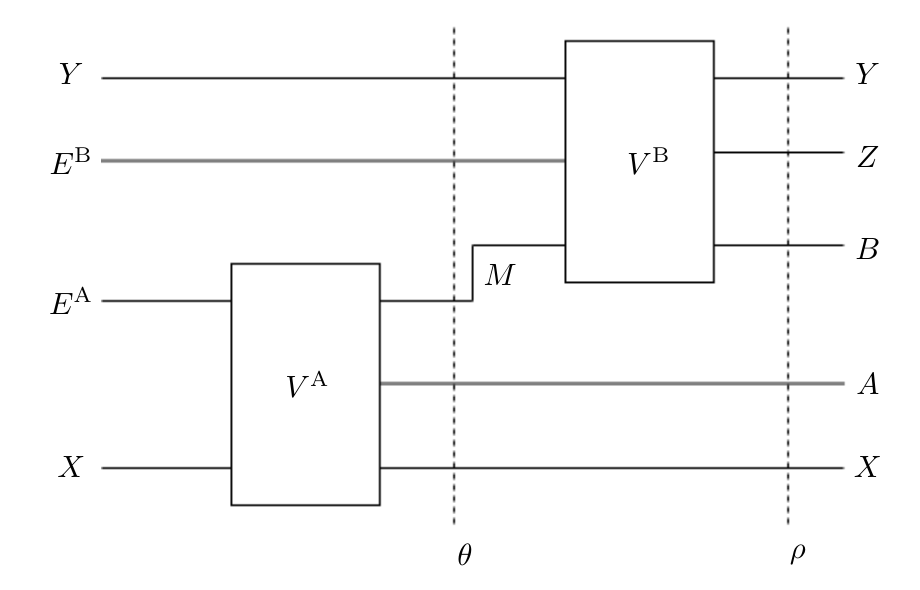
\includegraphics[width=0.72\linewidth]{figure1.png}\\Figure1. One-way quantum protocol $\mathcal P$.\end{center}

\section*{Author Section 3.2: proof of Theorem 1}
We show that if $ck<\zeta^5kQ^1_{p,\epsilon+12\zeta}(\widetilde f)/300-k\log\log(24/(5\zeta))$, the success of $\mathcal P$ is $(1-\epsilon)^{\Omega(\zeta^6k/\log|\mathcal Z|)}$.
\paragraph{Lemma 31.} Let $\delta=\zeta^6/1440000$, $\delta'=\zeta^6/(1440000\log|\mathcal Z|)$. Let $T_i$ indicate correctness of $\mathcal P$ on $f(X_i,Y_i)$. If its communication is $<\zeta^5kQ^1_{p,\epsilon+12\zeta}(\widetilde f)/60-k\log\log(24/(5\zeta))$, there exist $\lfloor\delta'k\rfloor$ coordinates $i_1,\ldots,i_{\lfloor\delta'k\rfloor}$ such that for all $1\le r\le\lfloor\delta'k\rfloor-1$ either
\[\Pr[\prod_{j=1}^rT_{i_j}=1]\le(1-\epsilon)^{\delta k},\]
or $\Pr[T_{i_{r+1}}=1\mid\prod_{j=1}^rT_{i_j}=1]\le1-\epsilon$.
Inductively suppose $C=\{i_1,\ldots,i_t\}$ has been found, $1\le t\le\lfloor\delta'k\rfloor$, with each conditional success at most $1-\epsilon$. Let $\mathcal E$ be $\prod_{i\in C}T_i=1$. If $\Pr[\mathcal E]\le(1-\epsilon)^{\delta k}$, done. Otherwise identify the next coordinate with conditional success at most $1-\epsilon$. The first coordinate is similar with empty conditioning; only the lower bound on conditioning probability is used.
Use $\ket\phi$, the state $\ket\rho$ conditioned on $\mathcal E$. For each $DG=dg$ define
\begin{multline*}\ket\phi_{X\widetilde XY\widetilde YABZ|dg}=\frac1{\sqrt{\gamma_{dg}}}\sum_{xy}\sqrt{P_{XY|dg}(xy)}\ket{xxyy}_{X\widetilde XY\widetilde Y}\\\otimes\sum_{z_C:(x_C,y_C,z_C)\in\widetilde f^t}\ket{z_C}_{Z_C}\ket{\widetilde\phi}_{ABZ_{\overline C}|xyz_C}.
\end{multline*}
The subnormalized state obeys $\|\ket{\widetilde\phi}_{ABZ_{\overline C}|xyz_C}\|_2^2=P_{Z_C|xy}(z_C)$. $\gamma_{dg}=\Pr[\mathcal E|dg]$ and $\sum_{dg}P_{DG}(dg)\gamma_{dg}=\Pr[\mathcal E]$. The distribution of $XYZ$ in this state is $P_{XYZ|\mathcal E,dg}$. Registers $DG$ are not explicitly considered: $\ket\phi_{dg}$ is notation without measuring such registers. Likewise $\ket\phi_{d_{-i}g_{-i}}$ conditions on $d_{-i}g_{-i}$ and changes only normalization. $\phi_{x_iy_id_{-i}g_{-i}}$ is obtained by measurement of the actual $X_iY_i$ registers. For $i\notin\overline C$, the authors use pure states $\ket\phi_{X_{\overline C}\widetilde X_{\overline C}Y_{\overline C}\widetilde Y_{\overline C}ABZ_{\overline C}|x_iy_ix_Cy_Cz_Cd_{-i}g_{-i}}$.
\paragraph{Lemma 32.} If $\Pr[\mathcal E]\ge(1-\epsilon)^{\delta k}$, there is $i\in\overline C$, $R_i=X_CY_CZ_CD_{-i}G_{-i}$, and for each $R_i=r_i$ a state $\ket{\phi'}_{X_{\overline C}\widetilde X_{\overline C}Y_{\overline C}\widetilde Y_{\overline C}ABZ_{\overline C}|y^*r_i}$ satisfying:
\begin{enumerate}\item[(i)] $\|P_{X_iY_iR_i|\mathcal E}-P_{X_iY_i}P_{R_i|\mathcal E,X_i}\|_1\le7\zeta/120$.
\item[(ii)] $\|P_{X_iY_iR_i|\mathcal E}-P_{X_iY_i}P_{R_i|\mathcal E,Y_i}\|_1\le7\zeta/120$.
\item[(iii)] There are projectors $\Pi_{x_ir_i}$ on $X_{\overline C}\widetilde X_{\overline C}A$ and unitaries $U_{y_ir_i}$ on $Y_{\overline C}\widetilde Y_{\overline C}BZ_{\overline C}$. Each projector succeeds on $\ket{\phi'}_{r_i}$ with probability $\alpha=2^{-c'}$, $c'\le60c/\zeta^5$, and
\begin{multline*}\mathbb E_{P_{X_iY_iR_i|\mathcal E}}\left[\left\|\frac1\alpha(\Pi_{x_ir_i}\otimes U_{y_ir_i})\proj{\phi'}_{y^*r_i}(\Pi_{x_ir_i}\otimes U_{y_ir_i}^\dagger)\right.\right.\\\left.\left.-\proj\phi_{x_iy_ir_i}\right\|_1\right]\le21\zeta.
\end{multline*}\end{enumerate}
Its complete author proof is in Section3.3 below.
\paragraph{Proof of Lemma 31.} Construct a protocol $\mathcal P'$ for $\widetilde f$ on distribution $P_{X_iY_i}=q$ by embedding inputs into the chosen state.
\begin{itemize}\item Alice/Bob have $r$ distributed as required by Fact12 as shared randomness, and $2^{60c/\zeta^5}\log(24/(5\zeta))$ copies of $\ket{\phi'}_{y^*r_i}$ as entanglement, Alice holding $X_{\overline C}\widetilde X_{\overline C}A$ and Bob the remaining registers.
\item On input $(x_i,y_i)$, Fact12 and Lemma32(i),(ii) give $R_i^A,R_i^B$ with
\[\|P_{X_iY_iR_i^AR_i^B}-P_{X_iY_iR_iR_i|\mathcal E}\|_1\le7\zeta/24,\]
where $R_iR_i$ are perfectly correlated copies.
\item Alice measures $\{\Pi_{x_ir_i^A},1-\Pi_{x_ir_i^A}\}$ on each copy. If none succeeds, abort. Otherwise send a $(60c/\zeta^5+\log\log(24/(5\zeta)))$-bit message indexing a successful copy.
\item Bob applies $U_{y_ir_i^B}$ on that copy and measures $Z_i$ for his output.\end{itemize}
By construction,
\[\mathbb E_{P_{X_iY_iR_i|\mathcal E}}\Pr[Z_i\text{ measured on }\ket\phi_{x_iy_ir_i}\in\widetilde f(x_i,y_i)]=\Pr[T_i=1|\mathcal E].\]
First suppose the inputs and $R_i^A,R_i^B$ follow exactly $P_{X_iY_iR_iR_i|\mathcal E}$, writing both copies $r_i$. The abort probability is
\[(1-2^{-c'})^{2^{60c/\zeta^5}\log(24/(5\zeta))}\le5\zeta/24.\]
If not aborting, the state after Bob's unitary is $\alpha^{-1/2}(\Pi_{x_ir_i}\otimes U_{y_ir_i})\ket{\phi'}_{y^*r_i}$. Lemma32(iii) gives expected correctness at least $\Pr[T_i=1|\mathcal E]-21\zeta/2$. Including abort, at least $\Pr[T_i=1|\mathcal E]-21\zeta/2-5\zeta/24$. For the actual $R_i^A,R_i^B$ distribution, success is at least
\[\Pr[T_i=1|\mathcal E]-21\zeta/2-5\zeta/24-7\zeta/24\ge\Pr[T_i=1|\mathcal E]-11\zeta.\]
Since $\|q-p\|_1\le2\zeta$, running this protocol on $p$ gives success $\ge\Pr[T_i=1|\mathcal E]-12\zeta$. Communication is $60c/\zeta^5+\log\log(24/(5\zeta))<Q^1_{p,\epsilon+12\zeta}(\widetilde f)$. If $\Pr[T_i=1|\mathcal E]\ge1-\epsilon$, error is $\le\epsilon+12\zeta$, a contradiction. Hence $\Pr[T_i=1|\mathcal E]\le1-\epsilon$. Take $i_{t+1}=i$.\qed

\section*{Complete author Section 3.3, distribution bounds}
First show in expectation over $i\in\overline C$ that distributions conditioned on $\mathcal E$ are close to unconditional ones. Fact10 with trivial $T,V$ and $U_i=X_iY_iD_iG_i$ gives
\[\mathbb E_{i\in\overline C}\|P_{X_iY_iD_iG_i|\mathcal E}-P_{X_iY_iD_iG_i}\|_1\le\frac1{k-t}\sqrt{k\log((1-\epsilon)^{-\delta k})}\le\sqrt{2\delta}.\tag{6}\]
By(5),
\[\mathbb E_{i\in\overline C}P_{Y_iG_i|\mathcal E,D_i=1}(Y_i=G_i)\ge1-\zeta/3-\sqrt{2\delta}.\tag{7}\]
Since $P_{G_i|D_i=1}(y^*)=1-(1-\zeta)^{2/3}$, and $P_{Y_i|D_i=1,G_i=y_i}(y_i)=(1-\zeta)^{1/3}$ for $y_i\in\mathcal Y$,
\begin{align*}\zeta+\sqrt{2\delta}&\ge1-(1-\zeta)^{2/3}+\sqrt{2\delta}\\&\ge\mathbb E_{i\in\overline C}P_{G_i|\mathcal E,D_i=1}(y^*)\\&\ge1-(1-\zeta)^{2/3}-\sqrt{2\delta}\ge2\zeta/3-\sqrt{2\delta},\tag{8}\end{align*}
and
\begin{align*}(1-\zeta/3+\sqrt{2\delta})\mathbb E_iP_{G_i|\mathcal E,D_i=1}(y_i)&\ge\mathbb E_iP_{Y_iG_i|\mathcal E,D_i=1}(y_i,y_i)\\&\ge(1-\zeta-\sqrt{2\delta})\mathbb E_iP_{G_i|\mathcal E,D_i=1}(y_i).\tag{9}\end{align*}
Use Fact10 again with $U_i=X_iY_i$, $T=X_CY_CDG$, $V=Z_C$. Set $\delta_1=\delta+\delta'\log|\mathcal Z|=\zeta^6/720000$. Then
\begin{align*}\sqrt{2\delta_1}&\ge\mathbb E_i\|P_{X_iY_iX_CY_CZ_CDG|\mathcal E}-P_{X_CY_CZ_CDG|\mathcal E}P_{X_iY_i|X_CY_CDG}\|_1\\&=\mathbb E_i\|P_{X_iY_iX_CY_CZ_CDG|\mathcal E}-P_{X_CY_CZ_CDG|\mathcal E}P_{X_iY_i|D_iG_i}\|_1\\&=\mathbb E_i\|P_{X_iY_iD_iG_iR_i|\mathcal E}-P_{D_iG_iR_i|\mathcal E}P_{X_iY_i|D_iG_i}\|_1.\tag{10}\end{align*}
$D_i$ is still uniform even conditioned on $\mathcal E$. From(10),
\begin{align*}\sqrt{2\delta_1}&\ge\tfrac12\mathbb E_i\|P_{X_iY_iG_iR_i|\mathcal E,D_i=0}-P_{G_iR_i|\mathcal E,D_i=0}P_{X_iY_i|G_i,D_i=0}\|_1\\&=\tfrac12\mathbb E_i\|P_{X_iY_iR_i|\mathcal E}-P_{X_iR_i|\mathcal E}P_{Y_i|X_i}\|_1,\end{align*}
since $X_i=G_i$ if $D_i=0$. Combine with $\mathbb E_i\|P_{X_i|\mathcal E}-P_{X_i}\|_1\le\sqrt{2\delta}$:
\[\mathbb E_i\|P_{X_iY_iR_i|\mathcal E}-P_{X_iY_i}P_{R_i|\mathcal E,X_i}\|_1\le3\sqrt{2\delta_1}<7\zeta^3/600.\tag{11}\]
Corollary9 gives
\[\mathbb E_i\|P_{X_iR_i|\mathcal E,y^*}-P_{X_iR_i|\mathcal E}\|_1\le33\sqrt{2\delta_1}/\zeta.\tag{12}\]
Let $F_i$ be $Y_i=G_i$. From(7), its conditional probability is at least $1-\zeta/3-\sqrt{2\delta}$ in expectation. Fact7 gives
\begin{align*}&\mathbb E_i\|P_{X_iY_iR_i|\mathcal E}-P_{Y_iR_i|\mathcal E}P_{X_i|Y_i}\|_1\\&=\mathbb E_i\|P_{X_iY_iG_iR_i|\mathcal E,D_i=1,F_i}-P_{G_iR_i|\mathcal E,D_i=1,F_i}P_{X_iY_i|G_iD_i=1,F_i}\|_1\\&\le6\mathbb E_i\|P_{X_iY_iD_iR_i|\mathcal E,D_i=1}-P_{G_iR_i|\mathcal E,D_i=1}P_{X_iY_i|G_iD_i=1}\|_1\le6\sqrt{2\delta_1}.\end{align*}
Using $\mathbb E_i\|P_{Y_i|\mathcal E}-P_{Y_i}\|_1\le\sqrt{2\delta}$ as before,
\[\mathbb E_i\|P_{X_iY_iR_i|\mathcal E}-P_{X_iY_i}P_{R_i|\mathcal E,Y_i}\|_1\le7\sqrt{2\delta_1}=7\zeta^3/600.\tag{13}\]

\section*{Complete author Lemma32 proof, projectors}
We show projectors $\Pi_{x_ir_i}$ take a soon-defined $\ket{\phi'}_{y^*r_i}$ close to $\ket\phi_{x_iy^*r_i}$. The message $M$ has $ck$ qubits. By Fact21 for each $DG=dg$ there is $\sigma_{M|dg}$ with
\[S_\infty(\theta_{XY\widetilde YE^BM|dg}\|\theta_{XY\widetilde YE^B|dg}\otimes\sigma_{M|dg})\le2ck.\]
By Fact20,
\[S_\infty(\rho_{XY\widetilde YBZ|dg}\|V^B(\theta_{XY\widetilde YE^B|dg}\otimes\sigma_{M|dg})(V^B)^\dagger)\le2ck.\]
Let
\[\psi_{X_{\overline C}\QBobRest|dg}:=\operatorname{Tr}_{Z_C}\left(V^B(\theta_{XYE^B|dg}\otimes\sigma_{M|x_Cy_Cdg})(V^B)^\dagger\right).\]
$\theta_{XY\widetilde YE^B|dg}\otimes\sigma_{M|dg}$ is product across $X$ and the rest; $V^B$ does not act on $X$. Hence $\psi$ is product across $X$ and the remaining registers, and all $X_i$ are mutually product. We have
\[S_\infty(\rho_{XY\widetilde YBZ_{\overline C}|dg}\|\psi_{XY\widetilde YBZ_{\overline C}|dg})\le2ck.\]
Facts22/19 imply
\begin{align*}&\mathbb E_{P_{X_CY_CZ_CDG|\mathcal E}}S(\phi_{X_{\overline C}\QBobRest|x_Cy_Cz_Cdg}\|\psi_{X_{\overline C}\QBobRest|x_Cy_Cdg})\\&\le\mathbb E_{P_{Z_CDG|\mathcal E}}S(\phi_{XY\widetilde YBZ_{\overline C}|z_Cdg}\|\psi_{XY\widetilde YBZ_{\overline C}|dg})\\&\le\mathbb E_{P_{Z_CDG|\mathcal E}}S_\infty(\phi_{XY\widetilde YBZ_{\overline C}|z_Cdg}\|\psi_{XY\widetilde YBZ_{\overline C}|dg})\\&\le\mathbb E_{P_{Z_CDG|\mathcal E}}\left[S_\infty(\phi_{XY\widetilde YBZ_{\overline C}|z_Cdg}\|\phi_{XY\widetilde YBZ_{\overline C}|dg})\right.\\&\qquad+S_\infty(\phi_{XY\widetilde YBZ_{\overline C}|dg}\|\rho_{XY\widetilde YBZ_{\overline C}|dg})\\&\qquad\left.+S_\infty(\rho_{XY\widetilde YBZ_{\overline C}|dg}\|\psi_{XY\widetilde YBZ_{\overline C}|dg})\right]\\&\le\mathbb E_{P_{Z_CDG|\mathcal E}}[\log(1/P_{Z_C|\mathcal E}(z_C))+\log(1/\Pr[\mathcal E])+2ck]\\&\le|C|\log|\mathcal Z|+\delta k+2ck\le(\delta_1+2c)k.
\end{align*}
By Quantum Raz's Lemma,
\begin{align*}4c+2\delta_1&\ge\mathbb E_i\mathbb E_{P_{X_CY_CZ_CDG|\mathcal E}}I(X_i:\QBobRest)_{\phi_{x_Cy_Cz_Cdg}}\\&=\mathbb E_i\mathbb E_{P_{D_iG_iR_i|\mathcal E}}I(X_i:\QBobRest)_{\phi_{d_ig_ir_i}}\\&\ge\mathbb E_i\tfrac12P_{G_i|\mathcal E,D_i=1}(y^*)\mathbb E_{P_{R_i|\mathcal E,D_i=1,G_i=y^*}}I(X_i:\QBobRest)_{\phi_{r_i|D_i=1,G_i=y^*}}\\&\ge\mathbb E_i\tfrac12(2\zeta/3-\sqrt{2\delta})\mathbb E_{P_{R_i|\mathcal E,D_i=1,G_i=y^*}}I(X_i:\QBobRest)_{\phi_{r_i,D_i=1,G_i=y^*}}.\tag{14}\end{align*}
Use(8) in the last step. The state $\phi_{\QAllRest|x_ir_i,D_i=1,G_i=y^*}$ is the same as $\phi_{\QAllRest|x_iy^*r_i}$, where $Y_i$, rather than $G_i$, is conditioned. $\ket\phi_{r_i,D_i=1,G_i=y^*}$ is the superposition over $X_i$ of those states with distribution $P_{X_i|\mathcal E,r_i,D_i=1,G_i=y^*}$. It differs from $\ket\phi_{y^*r_i}$ only in that distribution, the latter using $P_{X_i|\mathcal E,y^*r_i}$. Abbreviate the former as $\ket\phi_{r_i,1,y^*}$; this is distinct from $\ket\phi_{y^*r_i}$. Use the same convention for distributions.
$P_{X_i|1,y^*}=P_{X_i|y^*}$ and $P_{R_i|\mathcal E,x_i,1,y^*}=P_{R_i|\mathcal E,x_iy^*}$. Hence
\begin{align*}&\mathbb E_i\|P_{X_iR_i|\mathcal E,y^*}-P_{X_iR_i|\mathcal E,1,y^*}\|_1\\&\le\mathbb E_i[\|P_{X_iR_i|\mathcal E,y^*}-P_{X_i|y^*}P_{R_i|\mathcal E,X_i,y^*}\|_1\\&\qquad+\|(P_{X_i|1,y^*}-P_{X_i|\mathcal E,1,y^*})P_{R_i|\mathcal E,X_i,y^*}\|_1]\\&\le\mathbb E_i\left[\frac{\|P_{X_iR_i|\mathcal E}-P_{X_i}P_{R_i|\mathcal E,X_i}\|_1}{2\zeta/3-\sqrt{2\delta}}+\frac{\|P_{X_i|\mathcal E}-P_{X_i}\|_1}{2\zeta/3-\sqrt{2\delta}}\right]\\&\le7\sqrt{2\delta_1}/\zeta.
\end{align*}
By this and(12), $\mathbb E_i\|P_{X_iR_i|\mathcal E}-P_{X_iR_i|\mathcal E,1,y^*}\|_1\le40\sqrt{2\delta_1}/\zeta$.
Define
\[\ket{\phi'}_{\QAllRest|y^*r_i}:=\sum_{x_i}\sqrt{P_{X_i|\mathcal E,r_i}}\ket\phi_{\QAllRest|x_iy^*r_i}.\]
It is the same as $\ket\phi_{y^*r_i}$ with $X_i$'s distribution unconditioned on $Y_i=y^*$. By(14) and Fact23,
\[\mathbb E_iP_{X_iR_i|\mathcal E}\left(S_\infty^\zeta(\phi'_{\QBobRest|x_iy^*r_i}\|\phi'_{\QBobRest|y^*r_i})>\frac{28(2c+\delta_1)+1}{\zeta^4}\right)\le\zeta+\frac{20\sqrt{2\delta_1}}\zeta.\]
Fact25 gives projectors on $\QAliceRest$ succeeding with probability $\alpha=2^{-c'}$, $c'=60c/\zeta^5$, on $\ket{\phi'}_{\QAllRest|y^*r_i}$, and
\begin{multline*}\mathbb E_i\mathbb E_{P_{X_iR_i|\mathcal E}}\left\|\frac1\alpha(\Pi_{x_ir_i}\otimes1)\proj{\phi'}_{y^*r_i}(\Pi_{x_ir_i}\otimes1)-\proj\phi_{x_iy^*r_i}\right\|_1\\\le3\zeta+\frac{40\sqrt{2\delta_1}}{\zeta^2}\le\frac{7\zeta}2.\tag{15}\end{multline*}

\section*{Complete author Lemma32 proof, unitaries and recombination}
Next construct $U_{y_ir_i}$ taking $\ket\phi_{y^*r_i,D_i=1,G_i=y_i}$ close to $\ket\phi_{y_ir_i,D_i=1,G_i=y_i}$. Arguments like those leading to(14), on Bob's side without the initial message-information step, upper-bound
\[\mathbb E_{P_{X_CY_CZ_CDG|\mathcal E}}S(\phi_{Y_{\overline C}\QAliceRest|x_Cy_Cz_Cdg}\|\rho_{Y_{\overline C}\QAliceRest|x_Cy_Cdg}).\]
Raz's lemma gives
\begin{align*}2\delta_1&\ge\mathbb E_i\mathbb E_{P_{D_iG_iR_i|\mathcal E}}I(Y_i:\QAliceRest)_{\phi_{d_ig_ir_i}}\\&\ge\mathbb E_i\tfrac12(1-\zeta-\sqrt{2\delta})\mathbb E_{P_{R_iG_i|\mathcal E,D_i=1,G_i\ne y^*}}I(Y_i:\QAliceRest)_{\phi_{r_i,D_i=1,g_i}}\\&=\mathbb E_i\tfrac12(1-\zeta-\sqrt{2\delta})\mathbb E_{P_{R_iG_iY_i|\mathcal E,D_i=1,G_i\ne y^*}}S(\phi_{\QAliceRest|y_i,D_i=1,g_i}\|\phi_{\QAliceRest|D_i=1,g_i})\\&\ge\mathbb E_i\tfrac12(1-\zeta-\sqrt{2\delta})\sum_{y_i\in\mathcal Y}\mathbb E_{P_{R_i|\mathcal E,D_i=1,G_i=y_i}}P_{G_i|\mathcal E,D_i=1}(y_i)\\&\quad\cdot\left[(1-\zeta-\sqrt{2\delta})\|\phi_{\QAliceRest|y_i,r_i,1,y_i}-\phi_{\QAliceRest|r_i,1,y_i}\|_1^2\right.\\&\qquad\left.+(\zeta/3-\sqrt{2\delta})\|\phi_{\QAliceRest|y^*,r_i,1,y_i}-\phi_{\QAliceRest|r_i,1,y_i}\|_1^2\right].\end{align*}
Use(9) and Pinsker in the last line. By triangle inequality,
\begin{align*}&\mathbb E_i\sum_{y_i\in\mathcal Y}\mathbb E_{P_{R_i|\mathcal E,1,y_i}}P_{G_i|\mathcal E,1}(y_i)\|\phi_{\QAliceRest|y_ir_i,1,y_i}-\phi_{\QAliceRest|y^*r_i,1,y_i}\|_1^2\\&\le\mathbb E_i\sum_{y_i\in\mathcal Y}\mathbb E_{P_{R_i|\mathcal E,1,y_i}}2P_{G_i|\mathcal E,1}(y_i)\\&\quad\cdot[\|\phi_{\QAliceRest|y_i,r_i,1,y_i}-\phi_{\QAliceRest|r_i,1,y_i}\|_1^2+\|\phi_{\QAliceRest|y^*,r_i,1,y_i}-\phi_{\QAliceRest|r_i,1,y_i}\|_1^2]\\&\le\frac{4\delta_1}{1-\zeta-\sqrt{2\delta}}\left(\frac1{1-\zeta-\sqrt{2\delta}}+\frac1{\zeta/3-\sqrt{2\delta}}\right)\le\frac{32\delta_1}\zeta.
\end{align*}
The full conditional states are pure, so Fuchs--van de Graaf and Uhlmann give unitaries on $\QBobRest$ with
\begin{multline*}\mathbb E_i\sum_{y_i\in\mathcal Y}\mathbb E_{P_{R_i|\mathcal E,1,y_i}}P_{G_i|\mathcal E,1}(y_i)\\\cdot\|\proj\phi_{y_ir_i,1,y_i}-(1\otimes U_{y_ir_i})\proj\phi_{y^*r_i,1,y_i}(1\otimes U_{y_ir_i}^\dagger)\|_1\le(32\delta_1/\zeta)^{1/4}.\tag{16}\end{multline*}
It remains to show $\Pi_{x_ir_i}\otimes U_{y_ir_i}$ maps $\ket{\phi'}_{y^*r_i}$ close to $\ket\phi_{x_iy_ir_i}$. First show the unitary takes $\ket\phi_{x_iy^*r_i}$ close to $\ket\phi_{x_iy_ir_i}$. Let $O_{X_i}$ measure $X_i$ and write its outcome in another register. Then
\begin{align*}O_{X_i}(\proj\phi_{y_ir_i,1,y_i})&=\sum_{x_i}P_{X_i|\mathcal E,y_ir_i,D_i=1,G_i=y_i}(x_i)\proj{x_i}\otimes\proj\phi_{x_iy_ir_i,1,y_i}\\&=\sum_{x_i}P_{X_i|\mathcal E,y_ir_i,D_i=1,G_i=y_i}(x_i)\proj{x_i}\otimes\proj\phi_{x_iy_ir_i},\\O_{X_i}(\proj\phi_{y^*r_i,1,y_i})&=\sum_{x_i}P_{X_i|\mathcal E,y^*r_i,D_i=1,G_i=y_i}(x_i)\proj{x_i}\otimes\proj\phi_{x_iy^*r_i}.\end{align*}
The extra $D_i,G_i$ conditions do not change the two fully conditioned states. Fact10 gives
\[\mathbb E_i\|P_{X_iG_iR_i|\mathcal E,1}-P_{G_iR_i|\mathcal E,1}P_{X_i|1,G_i}\|_1\le2\sqrt{2\delta_1}.\]
Hence for any value $Y_i=y_i$,
\begin{align*}&\mathbb E_i\|P_{X_iG_iR_i|\mathcal E,1}-P_{G_iR_i|\mathcal E,1}P_{X_i|\mathcal E,y_i,1,G_iR_i}\|_1\\&\le\mathbb E_i[\|P_{X_iG_iR_i|\mathcal E,1}-P_{G_iR_i|\mathcal E,1}P_{X_i|y_i,1,G_i}\|_1\\&\qquad+\|P_{G_iR_i|\mathcal E,1}(P_{X_i|y_i,1,G_i}-P_{X_i|\mathcal E,y_i,1,G_iR_i})\|_1]\\&\le\mathbb E_i\left[\|P_{X_iG_iR_i|\mathcal E,1}-P_{G_iR_i|\mathcal E,1}P_{X_i|1,G_i}\|_1\right.\\&\qquad\left.+\frac2{\zeta/3-\sqrt{2\delta}}\|P_{X_iG_iR_i|\mathcal E,1}-P_{G_iR_i|\mathcal E,1}P_{X_i|1,G_i}\|_1\right]\\&\le8\sqrt{2\delta_1}/\zeta.
\end{align*}
Here $P_{Y_i|1,g_i}(y_i)\ge\zeta/3-\sqrt{2\delta}$ for every $G_i=g_i$. Also
\[\mathbb E_i\|P_{X_iG_iR_i|\mathcal E,1}-P_{X_iY_iR_i|\mathcal E,1}\|_1\le2P_{Y_iG_i|\mathcal E,1}(Y_i\ne G_i)\le\zeta/3+\sqrt{2\delta}.\]
Since $P_{X_iY_iR_i|\mathcal E,1}=P_{X_iY_iR_i|\mathcal E}$,
\[\mathbb E_i\|P_{X_iY_iR_i|\mathcal E}-P_{G_iR_i|\mathcal E,1}P_{X_i|\mathcal E,y_i,1,G_iR_i}\|_1\le8\sqrt{2\delta_1}/\zeta+\zeta/3+\sqrt{2\delta}.\]
Using this with(16),
\begin{align*}&\mathbb E_i\mathbb E_{P_{X_iY_iR_i|\mathcal E}}\|\proj\phi_{x_iy_ir_i}-(1\otimes U_{y_ir_i})\proj\phi_{x_iy^*r_i}(1\otimes U_{y_ir_i}^\dagger)\|_1\\&\le\mathbb E_i\left[\|P_{X_iY_iR_i|\mathcal E}-P_{G_iR_i|\mathcal E,1}P_{X_i|\mathcal E,y_i,1,G_iR_i}\|_1\right.\\&\quad+\|P_{X_iY_iR_i|\mathcal E}-P_{G_iR_i|\mathcal E,1}P_{X_i|\mathcal E,y^*,1,G_iR_i}\|_1\\&\quad+\mathbb E_{P_{G_iR_i|\mathcal E,1}}\left\|\mathbb E_{P_{X_i|\mathcal E,y_ir_i,1,y_i}}\proj{x_i}\otimes\proj\phi_{x_iy_ir_i}\right.\\&\qquad\left.\left.-\mathbb E_{P_{X_i|\mathcal E,y^*r_i,1,y_i}}(1\otimes U_{y_ir_i})\proj\phi_{x_iy^*r_i}(1\otimes U_{y_ir_i}^\dagger)\right\|_1\right]\\&=16\sqrt{2\delta_1}/\zeta+2\zeta/3+2\sqrt{2\delta}+(32\delta_1/\zeta)^{1/4}<7\zeta/10.\tag{17}\end{align*}
The last term is bounded by Fact15 applied to(16) with $O_{X_i}$. Conditioning on $G_i\ne y^*$ has also been removed: if $G_i=y^*$, both states are $\ket\phi_{x_iy^*r_i}$.
From(15),(17), triangle inequality gives
\begin{align*}&\mathbb E_i\mathbb E_{P_{X_iY_iR_i|\mathcal E}}\left\|\frac1\alpha(\Pi_{x_ir_i}\otimes U_{y_ir_i})\proj{\phi'}_{y^*r_i}(\Pi_{x_ir_i}\otimes U_{y_ir_i}^\dagger)-\proj\phi_{x_iy_ir_i}\right\|_1\\&\le\mathbb E_i\mathbb E_{P_{X_iY_iR_i|\mathcal E}}\left[\left\|\frac1\alpha(\Pi_{x_ir_i}\otimes U_{y_ir_i})\proj{\phi'}_{y^*r_i}(\Pi_{x_ir_i}\otimes U_{y_ir_i}^\dagger)\right.\right.\\&\qquad\left.-(1\otimes U_{y_ir_i})\proj\phi_{x_iy^*r_i}(1\otimes U_{y_ir_i}^\dagger)\right\|_1\\&\quad\left.+\|(1\otimes U_{y_ir_i})\proj\phi_{x_iy^*r_i}(1\otimes U_{y_ir_i}^\dagger)-\proj\phi_{x_iy_ir_i}\|_1\right]\\&=\mathbb E_i\mathbb E_{P_{X_iY_iR_i|\mathcal E}}\left[\left\|\frac1\alpha(\Pi_{x_ir_i}\otimes1)\proj{\phi'}_{y^*r_i}(\Pi_{x_ir_i}\otimes1)-\proj\phi_{x_iy^*r_i}\right\|_1\right.\\&\quad\left.+\|(1\otimes U_{y_ir_i})\proj\phi_{x_iy^*r_i}(1\otimes U_{y_ir_i}^\dagger)-\proj\phi_{x_iy_ir_i}\|_1\right]\\&\le7\zeta/2+7\zeta/10=21\zeta/5.\tag{18}\end{align*}
Markov's inequality on(11),(13),(18) gives an index $i\in\overline C$ satisfying all three conditions of Lemma32. This completes its proof, and hence the author's direct-product proof.\qed

\begin{thebibliography}{99}
\bibitem{ref1} Ziv Bar-Yossef, T. S. Jayram, Ravi Kumar, and D. Sivakumar. An Information Statistics Approach to Data Stream and Communication Complexity. In Proceedings of the 43th Annual IEEE Symposium on Foundations of Computer Science, FOCS ’02, pages 209–218, 2002. doi:10.1109/SFCS.2002.1181944.
\bibitem{ref2} Boaz Barak, Mark Braverman, Xi Chen, and Anup Rao. How to Compress Interactive Com- munication. SIAM Journal on Computing, 42(3):1327–1363, 2013. doi:10.1137/100811969.
\bibitem{ref3} Mohammad Bavarian, Thomas Vidick, and Henry Yuen. Anchoring Games for Parallel Repetition, 2015. arXiv:1509.07466.
\bibitem{ref4} Mohammad Bavarian, Thomas Vidick, and Henry Yuen. Hardness Amplification for Entangled Games via Anchoring. In Proceedings of the 49th Annual ACM SIGACT Symposium on Theory of Computing, STOC ’17, page 303–316, 2017. doi:10.1145/3055399.3055433.
\bibitem{ref5} Avraham Ben-Aroya, Oded Regev, and Ronald de Wolf. A Hypercontractive Inequality for Matrix-Valued Functions with Applications to Quantum Computing and LDCs. In Proceedings of the 49th Annual IEEE Symposium on Foundations of Computer Science, FOCS ’08, pages 477–486, 2008. doi:10.1109/FOCS.2008.45.
\bibitem{ref6} Mario Berta, Matthias Christandl, and Renato Renner. The Quantum Reverse Shannon Theorem Based on One-Shot Information Theory. Communications in Mathematical Physics, 306(3):579–615, 2011. doi:10.1007/s00220-011-1309-7.
\bibitem{ref7} Mark Braverman. Interactive information complexity. SIAM Journal on Computing, 44(6):1698– 1739, 2015. doi:10.1137/130938517.
\bibitem{ref8} Mark Braverman, Ankit Garg, Young Kun Ko, Jieming Mao, and Dave Touchette. Near- Optimal Bounds on Bounded-Round Quantum Communication Complexity of Disjointness. In 2015 IEEE 56th Annual Symposium on Foundations of Computer Science, pages 773–791, 2015. doi:10.1109/FOCS.2015.53.
\bibitem{ref9} Mark Braverman and Gillat Kol. Interactive Compression to External Information. In Proceedings of the 50th Annual ACM SIGACT Symposium on Theory of Computing, STOC ’18, page 964–977, 2018. doi:10.1145/3188745.3188956.
\bibitem{ref10} Mark Braverman and Anup Rao. Information Equals Amortized Communication. IEEE Trans- actions on Information Theory, 60(10):6058–6069, 2014. doi:10.1109/TIT.2014.2347282.
\bibitem{ref11} Mark Braverman, Anup Rao, Omri Weinstein, and Amir Yehudayoff. Direct Product via Round-Preserving Compression. In Automata, Languages, and Programming, volume 7965 of Lecture Notes in Computer Science, pages 232–243. Springer Berlin Heidelberg, 2013. doi:10.1007/978-3-642-39206-1\_20.
\bibitem{ref12} Mark Braverman, Anup Rao, Omri Weinstein, and Amir Yehudayoff. Direct Products in Communication Complexity. In Proceedings of the 54th Annual IEEE Symposium on Foundations of Computer Science, FOCS ’13, pages 746–755, 2013. doi:10.1109/FOCS.2013. 85.
\bibitem{ref13} Mark Braverman and Omri Weinstein. An Interactive Information Odometer and Applications. In Proceedings of the Forty-Seventh Annual ACM Symposium on Theory of Computing, STOC ’15, page 341–350, 2015. doi:10.1145/2746539.2746548.
\bibitem{ref14} Amit Chakrabarti, Yaoyun Shi, Anthony Wirth, and Andrew Yao. Informational Complexity and the Direct Sum Problem for Simultaneous Message Complexity. In Proceedings of the 42nd Annual IEEE Symposium on Foundations of Computer Science, FOCS ’01, pages 270–278, 2001. doi:10.1109/SFCS.2001.959901.
\bibitem{ref15} Richard Cleve, William Slofstra, Falk Unger, and Sarvagya Upadhyay. Perfect Parallel Repetition Theorem for Quantum XOR Proof Systems. Computational Complexity, 17(2):282– 299, 2008. doi:10.1007/s00037-008-0250-4.
\bibitem{ref16} Irit Dinur. The PCP Theorem by Gap Amplification. J. ACM, 54(3):12–es, 2007. doi: 10.1145/1236457.1236459.
\bibitem{ref17} Irit Dinur, David Steurer, and Thomas Vidick. A Parallel Repetition Theorem for En- tangled Projection Games. Computational Complexity, 24(2):201–254, 2015. doi:10.1007/ s00037-015-0098-3.
\bibitem{ref18} Prahladh Harsha, Rahul Jain, David McAllester, and Jaikumar Radhakrishnan. The Commu- nication Complexity of Correlation. IEEE Transactions on Information Theory, 56(1):438–449, 2010.
\bibitem{ref19} Thomas Holenstein. Parallel Repetition: Simplifications and the No-Signaling Case. In Proceedings of the Thirty-Ninth Annual ACM Symposium on Theory of Computing, STOC ’07, page 411–419, 2007. doi:10.1145/1250790.1250852.
\bibitem{ref20} Rahul Jain. New Strong Direct Product Results in Communication Complexity. Journal of the ACM, 62(3), 2015. doi:10.1145/2699432.
\bibitem{ref21} Rahul Jain and Hartmut Klauck. New Results in the Simultaneous Message Passing Model via Information Theoretic Techniques. In Proceedings of the 24th Annual IEEE Conference on Computational Complexity, CCC ’09, pages 369–378, 2009. doi:10.1109/CCC.2009.28.
\bibitem{ref22} Rahul Jain, Hartmut Klauck, and Ashwin Nayak. Direct Product Theorems for Classical Communication Complexity via Subdistribution Bounds: Extended Abstract. In Proceedings of the 40th Annual ACM Symposium on Theory of Computing, STOC ’08, pages 599–608, 2008. doi:10.1145/1374376.1374462.
\bibitem{ref23} Rahul Jain and Ashwin Nayak. Short Proofs of the Quantum Substate Theorem. IEEE Transactions on Information Theory, 58(6):3664–3669, 2012.
\bibitem{ref24} Rahul Jain, Attila Pereszlényi, and Penghui Yao. A Parallel Repetition Theorem for Entangled Two-Player One-Round Games under Product Distributions. In 2014 IEEE 29th Conference on Computational Complexity (CCC ’14), pages 209–216, 2014.
\bibitem{ref25} Rahul Jain, Attila Pereszlényi, and Penghui Yao. A Direct Product Theorem for Two-Party Bounded-Round Public-Coin Communication Complexity. Algorithmica, 76(3):720–748, 2016. doi:10.1007/s00453-015-0100-0.
\bibitem{ref26} Rahul Jain, Jaikumar Radhakrishnan, and Pranab Sen. The Quantum Communication Complexity of the Pointer Chasing Problem: The Bit Version. In FSTTCS 2002: Foundations of Software Technology and Theoretical Computer Science, volume 2556 of Lecture Notes in Computer Science, pages 218–229, 2002. doi:10.1007/3-540-36206-1\_20.
\bibitem{ref27} Rahul Jain, Jaikumar Radhakrishnan, and Pranab Sen. A Direct Sum Theorem in Com- munication Complexity via Message Compression. In Automata, Languages and Program- ming, volume 2719 of Lecture Notes in Computer Science, pages 300–315. Springer, 2003. doi:10.1007/3-540-45061-0\_26.
\bibitem{ref28} Rahul Jain, Jaikumar Radhakrishnan, and Pranab Sen. A Lower Bound for the Bounded Round Quantum Communication Complexity of Set Disjointness. In Proceedings of the 44th Annual IEEE Symposium on Foundations of Computer Science, FOCS ’03, pages 220–229. IEEE Computer Society, 2003. doi:10.1109/SFCS.2003.1238196.
\bibitem{ref29} Rahul Jain, Jaikumar Radhakrishnan, and Pranab Sen. Prior Entanglement, Message Com- pression and Privacy in Quantum Communication. In 20th Annual IEEE Conference on Computational Complexity (CCC ’05), pages 285–296, 2005.
\bibitem{ref30} Rahul Jain, Jaikumar Radhakrishnan, and Pranab Sen. Optimal Direct Sum and Privacy Trade- off Results for Quantum and Classical Communication Complexity, 2008. arXiv:0807.1267.
\bibitem{ref31} Rahul Jain, Jaikumar Radhakrishnan, and Pranab Sen. A Property of Quantum Relative Entropy with an Application to Privacy in Quantum Communication. Journal of the ACM, 56(6), 2009. doi:10.1145/1568318.1568323.
\bibitem{ref32} Rahul Jain and Penghui Yao. A Strong Direct Product Theorem in Terms of the Smooth Rectangle Bound, 2012. arXiv:1209.0263.
\bibitem{ref33} Zhengfeng Ji, Anand Natarajan, Thomas Vidick, John Wright, and Henry Yuen. MIP*=RE, 2020. arXiv:2001.04383.
\bibitem{ref34} Julia Kempe, Oded Regev, and Ben Toner. Unique Games with Entangled Provers are Easy. SIAM Journal on Computing, 39(7):3207–3229, 2010. doi:10.1137/090772885.
\bibitem{ref35} Hartmut Klauck. A Strong Direct Product Theorem for Disjointness. In Proceedings of the 42nd ACM Symposium on Theory of Computing, STOC ’10, pages 77–86, 2010. doi: 10.1145/1806689.1806702.
\bibitem{ref36} Hartmut Klauck, Robert Špalek, and Ronald de Wolf. Quantum and Classical Strong Direct Product Theorems and Optimal Time-Space Tradeoffs. SIAM Journal on Computing, 36(5):1472–1493, 2007. doi:10.1137/05063235X.
\bibitem{ref37} Gillat Kol. Interactive Compression for Product Distributions. In Proceedings of the Forty- Eighth Annual ACM Symposium on Theory of Computing, STOC ’16, page 987–998, 2016. doi:10.1145/2897518.2897537.
\bibitem{ref38} Troy Lee, Adi Shraibman, and Robert Špalek. A Direct Product Theorem for Discrepancy. In Proceedings of the 23rd Annual IEEE Conference on Computational Complexity, CCC ’08, pages 71–80, 2008. doi:10.1109/CCC.2008.25.
\bibitem{ref39} Ran Raz. A Parallel Repetition Theorem. In Proceedings of the Twenty-Seventh Annual ACM Symposium on Theory of Computing, page 447–456, 1995. doi:10.1145/225058.225181.
\bibitem{ref40} Alexander A. Razborov. On the Distributional Complexity of Disjointness. Theoretical Computer Science, 106(2):385–390, 1992. doi:10.1016/0304-3975(92)90260-M.
\bibitem{ref41} Ronen Shaltiel. Towards Proving Strong direct Product Theorems. Computational Complexity, 12(1-2):1–22, 2003. doi:10.1007/s00037-003-0175-x.
\bibitem{ref42} Alexander A. Sherstov. Strong Direct Product Theorems for Quantum Communication and Query Complexity. SIAM Journal on Computing, 41(5):1122–1165, 2012. doi:10.1137/ 110842661.
\bibitem{ref43} Alexander A. Sherstov. Compressing Interactive Communication Under Product Distributions. SIAM Journal on Computing, 47(2):367–419, 2018. doi:10.1137/16M109380X.
\bibitem{ref44} Emanuele Viola and Avi Wigderson. Norms, XOR Lemmas, and Lower Bounds for Polynomials and Protocols. Theory of Computing, 4(7):137–168, 2008. doi:10.4086/toc.2008.v004a007.
\bibitem{ref45} Andrew Chi-Chin Yao. Probabilistic computations: Toward a unified measure of complexity. In 18th Annual Symposium on Foundations of Computer Science (SFCS 1977), pages 222–227, 1977. doi:10.1109/SFCS.1977.24.
\bibitem{ref46} Henry Yuen. A Parallel Repetition Theorem for All Entangled Games. In 43rd International Colloquium on Automata, Languages, and Programming (ICALP ’16), volume 55 of Leibniz International Proceedings in Informatics (LIPIcs), pages 77:1–77:13, 2016. doi:10.4230/ LIPIcs.ICALP.2016.77.
\end{thebibliography}
\end{document}
